\documentclass[10pt, a5paper]{article}
\usepackage{pdfpages}
\usepackage{parallel}
\usepackage[T2A]{fontenc}
\usepackage{ucs}
\usepackage[utf8x]{inputenc}
\usepackage[polish,english,russian]{babel}
\usepackage{hyperref}
\usepackage{rotating}
\usepackage[inner=2cm,top=1.8cm,outer=2cm,bottom=2.3cm,nohead]{geometry}
\usepackage{listings}
\usepackage{graphicx}
\usepackage{wrapfig}
\usepackage{longtable}
\usepackage{indentfirst}
\usepackage{array}
\newcolumntype{P}[1]{>{\raggedright\arraybackslash}p{#1}}
\frenchspacing
\usepackage{fixltx2e} %text sub- and superscripts
\usepackage{icomma} % коскі ў матэматычным рэжыме
\PreloadUnicodePage{4}

\newcommand{\longpage}{\enlargethispage{\baselineskip}}
\newcommand{\shortpage}{\enlargethispage{-\baselineskip}}

\def\switchlang#1{\expandafter\csname switchlang#1\endcsname}
\def\switchlangbe{
\let\saverefname=\refname%
\def\refname{Літаратура}%
\def\figurename{Іл.}%
}
\def\switchlangen{
\let\saverefname=\refname%
\def\refname{References}%
\def\figurename{Fig.}%
}
\def\switchlangru{
\let\saverefname=\refname%
\let\savefigurename=\figurename%
\def\refname{Литература}%
\def\figurename{Рис.}%
}

\hyphenation{admi-ni-stra-tive}
\hyphenation{ex-pe-ri-ence}
\hyphenation{fle-xi-bi-li-ty}
\hyphenation{Py-thon}
\hyphenation{ma-the-ma-ti-cal}
\hyphenation{re-ported}
\hyphenation{imp-le-menta-tions}
\hyphenation{pro-vides}
\hyphenation{en-gi-neering}
\hyphenation{com-pa-ti-bi-li-ty}
\hyphenation{im-pos-sible}
\hyphenation{desk-top}
\hyphenation{elec-tro-nic}
\hyphenation{com-pa-ny}
\hyphenation{de-ve-lop-ment}
\hyphenation{de-ve-loping}
\hyphenation{de-ve-lop}
\hyphenation{da-ta-ba-se}
\hyphenation{plat-forms}
\hyphenation{or-ga-ni-za-tion}
\hyphenation{pro-gramming}
\hyphenation{in-stru-ments}
\hyphenation{Li-nux}
\hyphenation{sour-ce}
\hyphenation{en-vi-ron-ment}
\hyphenation{Te-le-pathy}
\hyphenation{Li-nux-ov-ka}
\hyphenation{Open-BSD}
\hyphenation{Free-BSD}
\hyphenation{men-ti-on-ed}
\hyphenation{app-li-ca-tion}

\def\progref!#1!{\texttt{#1}}
\renewcommand{\arraystretch}{2} %Іначай формулы ў матрыцы зліпаюцца з лініямі
\usepackage{array}

\def\interview #1 (#2), #3, #4, #5\par{

\section[#1, #3, #4]{#1 -- #3, #4}
\def\qname{LVEE}
\def\aname{#1}
\def\q ##1\par{{\noindent \bf \qname: ##1 }\par}
\def\a{{\noindent \bf \aname: } \def\qname{L}\def\aname{#2}}
}

\def\interview* #1 (#2), #3, #4, #5\par{

\section*{#1\\{\small\rm #3, #4. #5}}

\def\qname{LVEE}
\def\aname{#1}
\def\q ##1\par{{\noindent \bf \qname: ##1 }\par}
\def\a{{\noindent \bf \aname: } \def\qname{L}\def\aname{#2}}
}

\begin{document}
\title{Introduction to distributed file systems. OrangeFS experience}
\author{Andrew Savchenko\footnote{Moscow, Russia; NRNU MEPhI; \url{bircoph@gmail.com}}}
\maketitle
\begin{abstract}
An introduction to the world of distributed file systems is presen\-ted with a humble attempt to categorize them. A problem of choice is
considered from the workload profile point of view, and some common issues and pitfalls are discussed. A practical OrangeFS experience is
given with tips and tricks for better performance.
\end{abstract}
\section*{Preface}

Why one needs a non-local file system? Goals may vary, but usually they arise from the need of:

\begin{itemize}
  \item a \emph{large} data storage;
  \item a \emph{high performance} data storage;
  \item \emph{redundant} and highly available solutions.
\end{itemize}

There are dozens of solutions available\cite{bib1}, and many of them are open source. But how to choose one you need? There is a lot of ambiguity and vagueness in this field, but let's try to sort it out.

Focusing on open source solutions, one can see they are usually sufficient for any needs and are used on the most high performance systems from Top-500\cite{bib2} list, especially in the top 50 of them.

\section*{Species of distributed file systems}

Even the term ``distributed'' is ambiguous itself. It may mean all kinds of file systems running on more than a single host (sense used in a title of this article), but it also means a subset of this common sense discussed below. It should be understandable, that there is no canonical definitions in this field, so terminology found in different sources may vary.

Every non-local file system (except for few exotic cases) may be roughly related to one of the following classes:

\begin{itemize}
  \item network file systems;
  \item clustered file systems;
  \item distributed file systems.
\end{itemize}

Of course, there is a large intersection between these sets. See fig. \ref{fig:Sav1} for details.

\begin{figure}[h]
  \centering
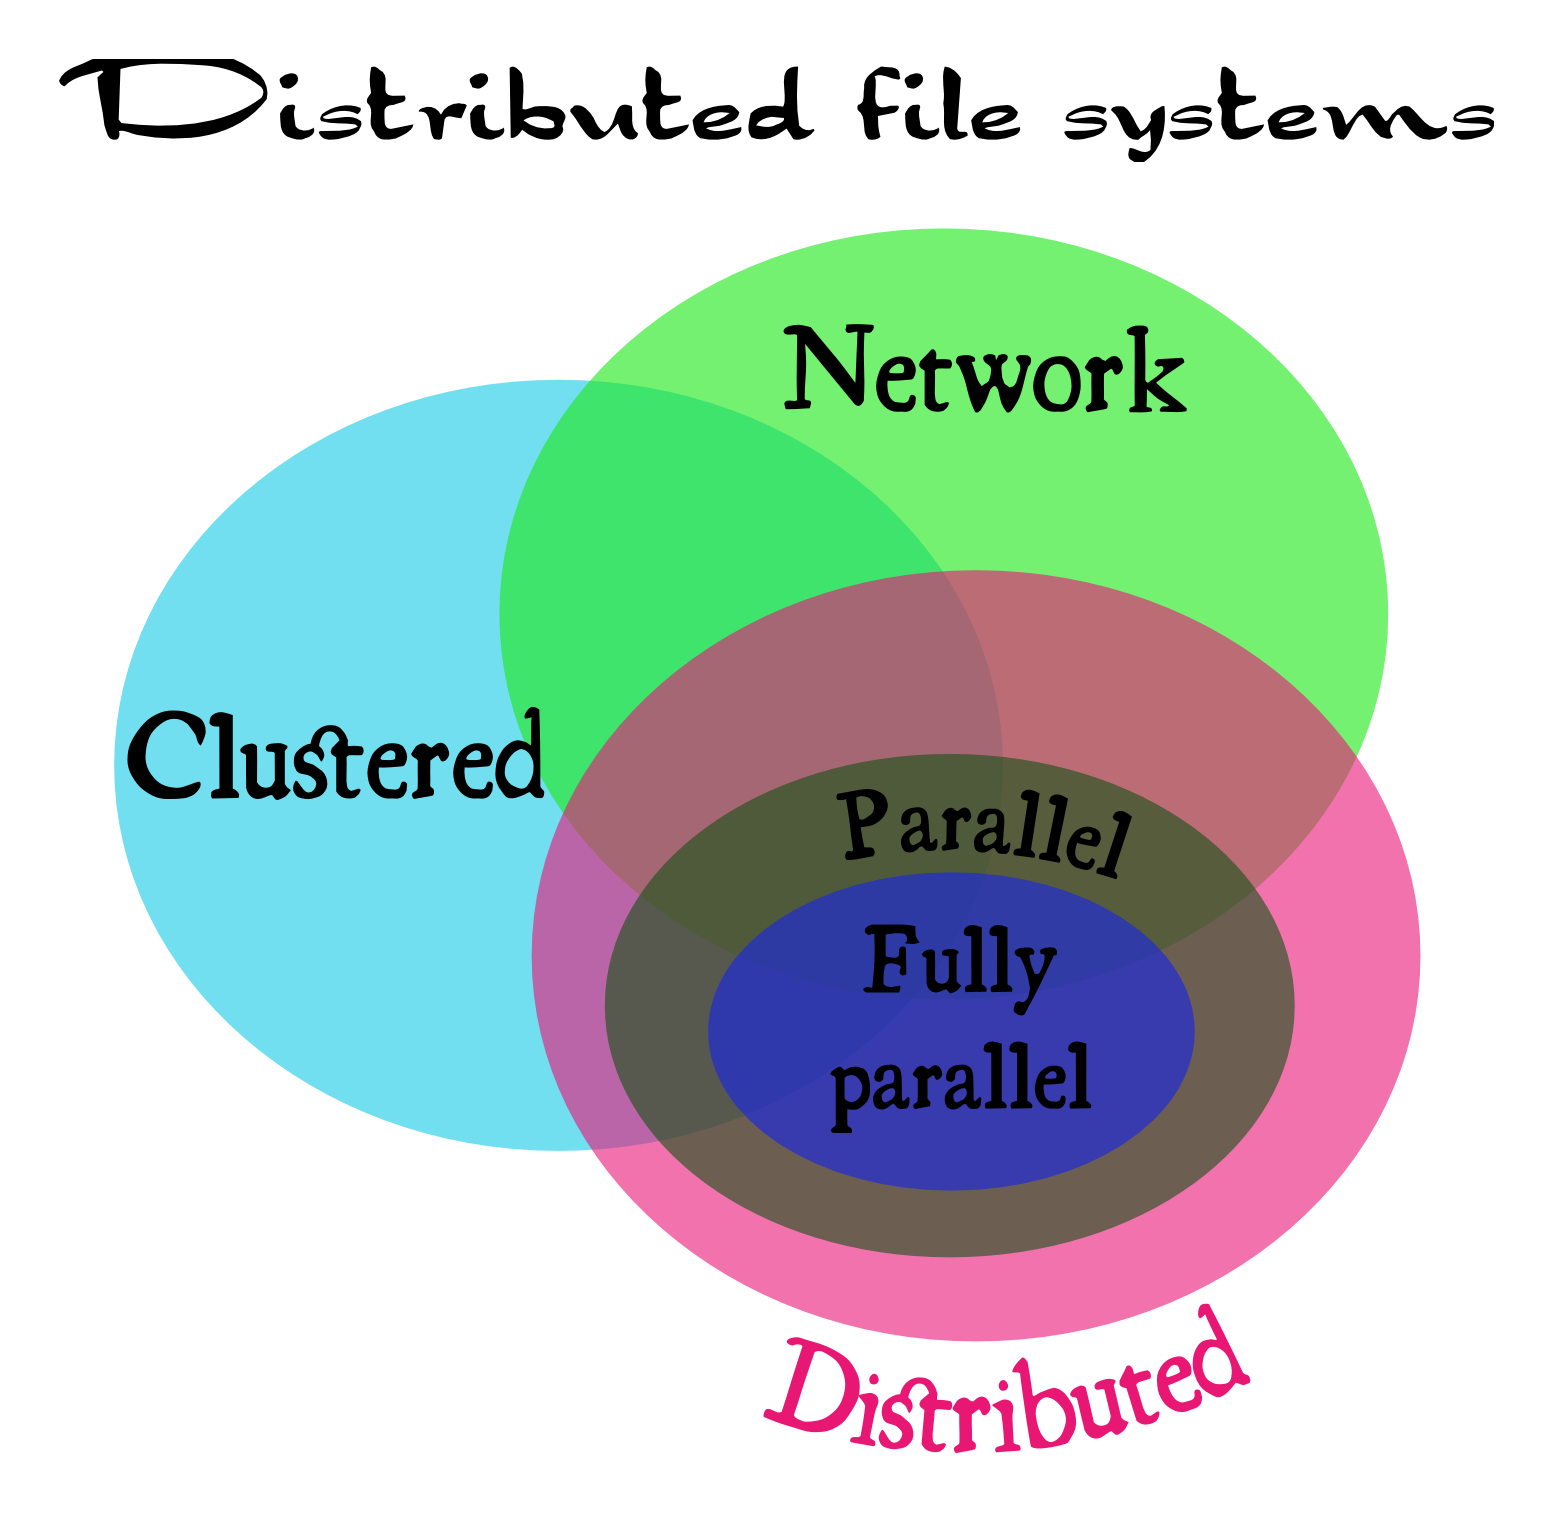
\includegraphics[height=4cm]{123_genesis.png}
\caption{Distributed flesystems}\label{fig:Sav1}
\end{figure}

\subsection*{Network file systems}

Network file system usually means one with a single server (or at least an appearance of a single server) and several remotely connected clients. Classical NFS\cite{bib3} is a good example (but not with pNFS\cite{bib4} extension).

\subsection*{Clustered file systems}

Clustered file system is a file system simultaneously mounted on several local servers sharing the same data storage on a block level (usually the SAN\cite{bib5} model is used). These kind of setups is called \emph{shared disk} file systems often. Well known examples are OCFS2\cite{bib6} and GFS2\cite{bib7} file systems.

\subsection*{Distributed file systems}

Distributed (in the narrow sense) file systems are setups with multiple data servers sharing nothing between them, for each active server its own data storage is private to it. This systems usually are not geographically distributed and are local in their location due to demands of high performance interconnect (e.g. pNFS\cite{bib3} extension of NFS\cite{bib2} falls here). But there are solutions present for geographically distributed systems, even for setups distributed across different continents. Andrew File System (AFS\cite{bib8}) is a good and widely used example.

\subsection*{Parallel file systems}

Whenever file system is called parallel, this means it provides a parallel access to (usually all of) its storage hosts for each of its clients. This allows to avoid a bottleneck of a single host in terms of both network and I/O bandwidth, latency; CPU and cache limitations. These file systems are usually used in the High Performance Computing (HPC\cite{bib2}\cite{bib9}) and high-end business applications like stock exchange information systems. Prominent open source examples are Lustre\cite{bib10}, OrangeFS\cite{bib11} and Ceph\cite{bib12}.

\subsubsection*{Fully parallel file systems}

Parallel file systems are fully parallel when not only data, but metadata is also distributed on multiple servers accessible in parallel by clients. This is quite important for high-end performance as single metadata server will eventually become a bottleneck, especially when dealing with large directories. For example, OrangeFS\cite{bib11} and Ceph\cite{bib12} are fully parallel distributed file systems, but pNFS\cite{bib4} ad Lustre\cite{bib10} are not.

\subsection*{Highly Available (HA) solutions}

Each class described above may contain an HA solution. Usually this is done by either a data replication (as in Ceph\cite{bib12}) or by a disk level redundancy (RAID5/6) together with a server level redundancy (heartbeat/pacemaker) as in Lustre\cite{bib10} or OrangeFS\cite{bib11}.

\subsection*{MPI support}

If you're working in the HPC\cite{bib9} field, you'll be definitely interested in the MPI\cite{bib13} I/O support. ROMIO\cite{bib14} implements just that and is supported by many file systems, e.g. NFS\cite{bib3}, Lustre\cite{bib10}, OrangeFS\cite{bib11}.

\section*{Setup considerations}

Final choise should be made based on targeted applications for your setup:

\begin{itemize}
  \item is POSIX compliance setup required? Especially POSIX file locking, it hinders greatly distributed file system performance (and is not available on many file systems at all), but may be required by some applications;
  \item is MPI\cite{bib13} needed?
  \item is HA needed?
  \item what kind of locality are you targeted on?
  \item are your data servers exclusive for your storage tasks?
  \item are you working in trusted environment?
  \item and many more\ldots{}
\end{itemize}

\emph{Optimize} your software:

\begin{itemize}
  \item prefer a small number of large files over a large number of small files, as large directories hinder metadata servers greatly;
  \item prefer large data chunks over a large number of small network packets — they hinder TCP/IP stack greatly.
\end{itemize}

\section*{OrangeFS experience}

At our university we selected OrangeFS because of the following:

\begin{itemize}
  \item parallel distributed FS with good MPI support;
  \item reasonable performance on large directories;
  \item optional HA support;
  \item low CPU load;
  \item high network I/O performance (limited only by physical 1 Gbit/s bandwidth);
  \item native InfiniBand\cite{bib15} support.
\end{itemize}

Though, high performance means non full POSIX compliance, so:

\begin{itemize}
  \item no hardlinks;
  \item no special files;
  \item no unlink(): if file is gone, then it is gone immediately and forever.
  \item OrangeFS should not be used for \$HOME.
\end{itemize}

Setup hints:

\begin{itemize}
  \item use as many data \emph{and} metadata servers as possible;
  \item use large stip\_size, 1 MB is a good idea to start with;
  \item TroveSync may be disabled to improve speed at the cost of possible data loss when server dies;
  \item on ethernet use jumbo frames.
\end{itemize}

This software is a good example of how ordinary user sends patches made due to daily needs and became a project contributor :)

\section*{Summary}

There is no perfect distributed filesystem: to achieve the best in one aspect some others must be sacrificed. But if you understand your workload, you'll be able to pick up a few solutions, study them to your best and have fun!

In my humble opinion the most interesting and promising solutions for their fields are: Lustre\cite{bib10}, OrangeFS\cite{bib11}, Ceph\cite{bib12} and pNFS\cite{bib4}.

P.S. Always send your patches!

\begin{thebibliography}{9}
\bibitem{bib1} {\href{http://en.wikipedia.org/wiki/List_of_file_systems}{http://en.wikipedia.org/wiki/List\_of\_file\_systems}}
\bibitem{bib2} {\href{http://www.top500.org/}{http://www.top500.org/}}
\bibitem{bib3} {\href{http://linux-nfs.org/}{http://linux-nfs.org/}}
\bibitem{bib4} {\href{http://www.pnfs.com/}{http://www.pnfs.com/}}
\bibitem{bib5} {\href{http://en.wikipedia.org/wiki/Storage_area_network}{http://en.wikipedia.org/wiki/Storage\_area\_network}}
\bibitem{bib6} {\href{https://oss.oracle.com/projects/ocfs2/}{https://oss.oracle.com/projects/ocfs2/}}
\bibitem{bib7} {\href{https://access.redhat.com/knowledge/docs/en-US/Red_Hat_Enterprise_Linux/6/html/Global_File_System_2/ch-overview-GFS2.html}{https://access.redhat.com/knowledge/docs/en-US/Red\_Hat\_Enterprise\_Linux/6/html/Global\_File\_System\_2/ch-overview-GFS2.html}}
\bibitem{bib8} {\href{http://www.openafs.org/}{http://www.openafs.org/}}
\bibitem{bib9} {\href{http://en.wikipedia.org/wiki/Supercomputer}{http://en.wikipedia.org/wiki/Supercomputer}}
\bibitem{bib10} {\href{http://lustre.org/}{http://lustre.org}}
\bibitem{bib11} {\href{http://www.orangefs.org/}{http://www.orangefs.org/}}
\bibitem{bib12} {\href{http://ceph.com/}{http://ceph.com/}}
\bibitem{bib13} {\href{http://en.wikipedia.org/wiki/Message_Passing_Interface}{http://en.wikipedia.org/wiki/Message\_Passing\_Interface}}
\bibitem{bib14} {\href{http://www.mcs.anl.gov/research/projects/romio/}{http://www.mcs.anl.gov/research/projects/romio/}}
\bibitem{bib15} {\href{http://en.wikipedia.org/wiki/InfiniBand}{http://en.wikipedia.org/wiki/InfiniBand}}\end{thebibliography}
\end{document}
